%%
%% This is file `sample-sigconf.tex',
%% generated with the docstrip utility.
%%
%% The original source files were:
%%
%% samples.dtx  (with options: `sigconf')
%%
%% IMPORTANT NOTICE:
%%
%% For the copyright see the source file.
%%
%% Any modified versions of this file must be renamed
%% with new filenames distinct from sample-sigconf.tex.
%%
%% For distribution of the original source see the terms
%% for copying and modification in the file samples.dtx.
%%
%% This generated file may be distributed as long as the
%% original source files, as listed above, are part of the
%% same distribution. (The sources need not necessarily be
%% in the same archive or directory.)
%%
%% The first command in your LaTeX source must be the \documentclass command.
\documentclass[sigconf,noacm]{acmart}
\settopmatter{printacmref=false} % Removes citation information below abstract
\renewcommand\footnotetextcopyrightpermission[1]{} % removes footnote with conference information in first column
\pagestyle{plain} % removes running headers
\usepackage{subcaption}
\usepackage{minted}

%%
%% \BibTeX command to typeset BibTeX logo in the docs
\AtBeginDocument{%
  \providecommand\BibTeX{{%
    \normalfont B\kern-0.5em{\scshape i\kern-0.25em b}\kern-0.8em\TeX}}}

%% Rights management information.  This information is sent to you
%% when you complete the rights form.  These commands have SAMPLE
%% values in them; it is your responsibility as an author to replace
%% the commands and values with those provided to you when you
%% complete the rights form.
\setcopyright{acmcopyright}
\copyrightyear{2018}
\acmYear{2018}
\acmDOI{10.1145/1122445.1122456}

%% These commands are for a PROCEEDINGS abstract or paper.
\acmConference[CS294 Project]{Building an RTL Coverage Proxy Model for RISC-V CPUs}
{}{}

\tolerance=1
\emergencystretch=\maxdimen
\hyphenpenalty=10000
\hbadness=10000

\begin{document}

\title{Building an RTL Coverage Proxy Model for RISC-V CPUs}

\author{Vighnesh Iyer}
\email{vighnesh.iyer@berkeley.edu}
\affiliation{%
\institution{UC Berkeley}}
  %\institution{The Th{\o}rv{\"a}ld Group}
  %\streetaddress{1 Th{\o}rv{\"a}ld Circle}
  %\city{Hekla}
  %\country{Iceland}}

\renewcommand{\shortauthors}{Vighnesh Iyer}

\begin{abstract}
RTL verification consumes the majority of time in the hardware design cycle, so there is interest in increasing the efficiency of existing dynamic verification methods.
Typical dynamic verification loops utilize a constrained random stimulus generator to drive a design-under-test, while checking for buggy states and trajectories, and collecting RTL coverage data.
It is usually impossible to exclude the possiblity of bugs altogether, so verification engineers focus on maximizing RTL coverage as a proxy for the thoroughness of their testing efforts.

We propose the design of an RTL coverage proxy model which aims to predict structural RTL coverage from pre-RTL-simulation features.
Such a model can be used to: 1) avoid the wasteful RTL simulation of redundant or inferior tests, 2) provide DV engineers with insights on correlations between their stimulus generator and coverage to help with constraint and bias tuning, and 3) make automatic random variable distribution tuning viable by bypassing slow RTL simulation.


%During the design process, a considerable amount of data is produced such as per-test RTL coverage from nightly random regressions.
%Those same tests are executed on fast functional models which also produce large amounts of data such as C++ coverage, logs, and transaction and execution traces.

%We propose the construction of an RTL coverage prediction model which can estimate RTL coverage from functional simulation, to direct test selection and hit coverage goals faster.

%During unit design, nightly random regressions provide considerable per-test coverage data.
%Closing coverage by running regression workloads and random stimulus takes a long time and must be repeated if the RTL were to change.

%Ideally one only needs to simulate the specific stimulus vectors that would be likely to hit any uncovered coverpoints.
%However, to determine the RTL coverage of any proposed test stimulus requires slow RTL simulation or human intuition.
\end{abstract}

\maketitle

\section{Background}

\subsection{Digital Hardware Design}

The vast majority of digital systems are built using synchronous digital circuits.
These circuits can be described with a simple abstraction, consisting of 1) state and 2) update rules.
The state of a digital circuit is just `a bunch of bitvectors' and the update rules specify how every state bitvector should be updated as a logic function of all the state bitvectors.
The state is updated according to the update rules on the rising ($0 \rightarrow 1$) edge of a special one-bit \textit{clock} signal, which continuously toggles from $0 \rightarrow 1 \rightarrow 0$ at a fixed frequency.

Of course, digital circuits are usually not closed systems, otherwise there would be no way to pass data into them or get data out.
In addition to state and update rules, digital circuits also have top-level (primary) inputs and outputs, which are also bitvectors.
The update rules are now functions of both the current state and the primary inputs.
The primary outputs are a function of the current state and the primary inputs in the most general case (allowing combinational coupling of primary inputs to outputs).

\subsubsection{Transition System Representation}
We can formally represent a synchronous digital circuit as a transition system $T$.

\begin{equation*}
  T = (S, I, PI, R, PO)
\end{equation*}

where,

\begin{itemize}
  \item $S = $ a set of state elements (bitvectors)
  \item $I = $ a set of initial state assignments
  \item $PI = $ a list of the top-level (primary) inputs (bitvectors) to the circuit
  \item $R = $ the transition relation or update rules $R: S \times PI \rightarrow S$
  \item $PO = $ a list of the top-level (primary) outputs (bitvectors) of the circuit and their update rule $PO: S \times PI$
\end{itemize}

\subsubsection{Hardware Design Languages}

Synchronous digital circuits can be described in several different hardware design languages (HDLs) that operate at different levels of abstraction (all the way from software-like algorithmic/imperative descriptions of desired circuit behavior, down to transistor-level netlists).
The HDL abstraction level that matches the transition system representation of a circuit is called register-transfer level (RTL).
The primitives in an RTL-level HDL are state elements, update rules, and ports, and these can be desugared to transition systems.

The vast majority of digital circuits are written at the RTL-level since it gives the designer precise control over the state and logic that will end up on the chip.
The most popular RTL-level HDL is Verilog (which can also represent lower levels of circuit abstraction such as gate-level or transistor-level).
Here is an example of Verilog code:

\begin{minted}{verilog}
module alu(input [7:0] a, b,
           input op, clk, output reg [8:0] o);
  always_ff @(posedge clk)
    if (op) o <= a + b;
    else    o <= a - b;
endmodule
\end{minted}

This describes a transition system with one state element \texttt{o}, a single update rule \texttt{o <= op ? (a+b) : (a-b)}, three primary inputs \texttt{(a, b, op)}, and one primary output \texttt{o} (which is driven directly by the state element).

\subsection{Digital Hardware Simulation}

Simulating a synchronous digital circuit is equivalent to simulating its underlying transition system.
Verilog simulators implement a function $s$:

\begin{equation*}
  s(T, PI_0, PI_1, \dots, PI_n) = (PO_0, PO_1, \dots PO_n)
\end{equation*}

where given a concrete binding of each primary input for $n$ clock cycles of simulation, the simulator will return a sequence of concrete bindings of each primary output.

In practice, RTL testbenches invoke the underlying simulator one clock cycle at a time, by providing primary inputs for one cycle, telling the simulator to execute the update rules, inspecting the primary outputs, and repeating this process.
A popular Verilog simulator that supports this mode of execution is Verilator, and we use it for our benchmarks.

\subsubsection{Coverage Collection}

Just like software instrumentation techniques enable one to see which code paths were explored at the source-level, there are instrumentation passes built into RTL simulators that enable coverage collection during the simulation.
Hardware coverage is split into two types: 1) structural and 2) functional.

Structural coverage refers to any coverpoint that can be defined from analyzing the RTL AST in isolation.
This includes line/condition coverage (similar to the equivalent in software), toggle coverage (which measures the number of times a bit toggles between 0 and 1 for registers and ports), and FSM coverage (which covers all the states and unique transitions for any FSMs in an RTL design).

Functional coverage refers to any coverpoint that describes a microarchitectural feature that a designer wants to see exercised: these coverpoints must be manually defined and are specific to the semantics of a given design.


\subsection{Digital Hardware Verification}

\begin{figure}
  %\centering
  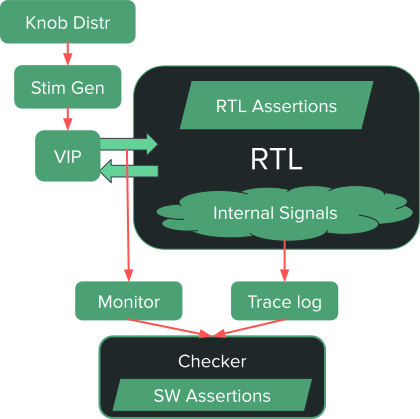
\includegraphics[width=0.65\linewidth]{figs/dynamic_verif.pdf}
  \caption{A typical dynamic verification environment}
  \label{fig:dynamic_verif}
\end{figure}

\subsubsection{Bug Identification}

Merely simulating a transition system by providing it with inputs doesn`t tell us if anything has gone wrong, since the simulation behavior is always well defined.
This is in contrast to user-space software which has `universal' modes of failure such as segfaults or stack overflows, which are failures that exist independently of the application logic itself.

In hardware verification, bugs are detected by manually written assertions in the Verilog RTL or by assertions that exist in the verification environment, most commonly comparing a software golden model of the hardware to the output of RTL simulation.
In the case of CPUs, bugs are detected by comparing the instruction commit logs between RTL simulation and ISA-level simulation, since instruction retirement is a synchronization point where we can expect a match in architectural state.

\subsubsection{Testbench Architecture}

See Figure \ref{fig:dynamic_verif} for the generic architecture of a verification environment.
A VIP (verification IP) is a component that can translate high-level transactions used to interact with the RTL design down to the low-level cycle-by-cycle and port-by-port representation the simulator understands.
The environment uses a stimulus generator to create random stimuli, which is driven into the RTL; internal signals from the RTL (e.g. PC register and register file) are inspected by other verification components and compared against a golden model.

\subsubsection{Stimulus Generators}

We usually do not write stimuli that interacts with an RTL design at its level of abstraction: by driving its primary inputs to the values we want and sampling its primary outputs.
Rather, we construct the stimuli at a higher level of abstraction and write a separate component (the VIP) that performs the abstraction translation.

This is the case for the verification of CPUs.
At the top-level of a CPU core, there is usually a memory interface that the core`s internal L1 caches will use to talk to the upper memory system.
If you wanted to simulate the execution of a program on the CPU, the testbench would have to manually drive the memory bus with the instructions and data from the program as the CPU requests them.
Our stimulus does not consist of these memory bus interactions, but rather only contains the assembly code we want the CPU to execute.

\subsubsection{The Anatomy of a Stimulus Generator}

The architecture of a CPU stimulus generator is shown in Figure \ref{fig:stimgen}.
A single stimulus is made up of a list of \textit{sequences}.
Each \textit{sequence} is a hand-crafted assembly generation template that aims to exercise some (micro)architectural feature of the CPU.

For instance, there might be a sequence for generating an arbitrary arithmetic instruction and another one for generating a group of assembly instructions that have a read-after-write (RAW) dependency.
Sequences can also refer to other sequences.
For instance, consider a loop sequence, which in turn will refer to another sequence to determine what goes into the loop body.

Sequences are assembly generators that need to sample sources of randomness (\textit{knobs}) to determine the concrete assembly they will emit.
For instance, the ``Any arithmetic inst'' sequence would sample the \textit{RInst} knob to determine which instruction to emit.
A knob defines a distribution over the values that knob can take on (for \textit{RInst}: a weight is assigned to every arithmetic instruction).
The same sequence would also need to sample the \textit{RegBinding} knob to determine which registers to use as the operands and destination.

While it would be ideal if stimulus generators were just a function of the knob distributions, in practice, these generators also consume a random seed.
This seed is used to: 1) seed a PRNG that can be sampled anytime inside the generator in addition to being used for sampling of knobs, and 2) seed the constraint solver sampler.
Most stimulus generators use declarative constraints that the underlying RTL simulator solves and samples from (see SystemVerilog`s support for constrained random stimulus generation).

\begin{figure}
  %\centering
  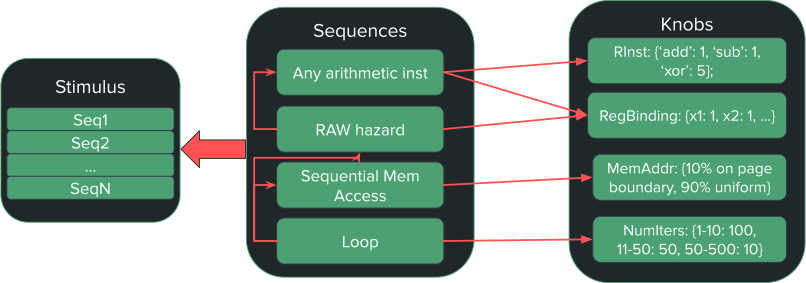
\includegraphics[width=1\linewidth]{figs/stimgen.pdf}
  \caption{The architecture of a CPU instruction generator}
  \label{fig:stimgen}
\end{figure}

\subsubsection{The Verification Loop}

\begin{figure}
  %\centering
  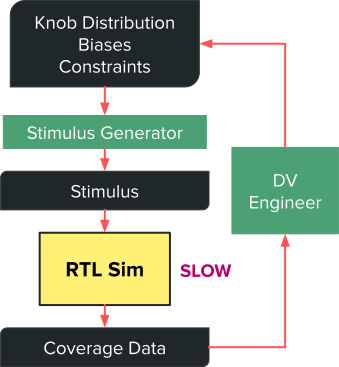
\includegraphics[width=0.65\linewidth]{figs/typical_verif_flow.pdf}
  \caption{A typical verification loop used in industry DV}
  \label{fig:verif_loop}
\end{figure}

The goal of any verification process is to find bugs.
Since it is impossible to rule out bugs on a large enough design, the practical goal becomes to close any coverage holes, or hit certain parts of the design harder to coax out any latent bugs.
This process is described in Figure \ref{fig:verif_loop} where a DV engineer inspects coverage data from RTL simulation and tunes knob distributions or adds new sequences to the generator to get the desired coverage.

The major limitation of this flow is that it is bottlenecked by the speed of RTL simulation which is often 10-100x slower than stimulus generation.
This long feedback latency motivates our technique.

\section{Proposed Technique}

In this project, we investigate whether it is viable to develop a coverage proxy model.
The proposed setup is shown in Figure \ref{fig:cov_proxy_model}.
The idea is by training a supervised model that can predict line coverage of RTL from the knob values passed into the stimulus generator, we enable a few potential functions:

\begin{enumerate}
  \item Stimulus pruning: there are many potential permutations of knob values that lead to similar generated stimulus with similar coverage characteristics. When running regressions, it would be useful to avoid wasting RTL simulation time on stimuli that aren`t likely to increase coverage.
  \item Correlation analysis: an interpretable coverage proxy model can show correlations between certain combinations of knobs and specific coverpoints. This data is useful for manual knob tuning and for validating the stimulus generator is targetting the coverpoints it ought to.
  \item Automated knob tuning: use the proxy model to make blackbox tuning viable; run RTL simulations only when needed to confirm expected coverage.
\end{enumerate}

\subsection{Experimental Setup}

We use riscv-dv, Google`s UVM-based RISC-V instruction generator as our stimulus generator.
riscv-dv has a total of 52 configurable knobs, of which only 23 are actually meaningful (and will not cause erroneous testbench failures) for the RV32IMC target configuration.
Of these 23, four are integer valued knobs and the other 19 are boolean 0/1 switches.
Here are a few of the knobs under consideration:

\begin{itemize}
  \item \verb|num_of_sub_program| (integer): Number of sequences (instruction streams) in the generated program
  \item \verb|instr_cnt| (integer): Total number of instructions in the final program
  \item \verb|no_branch_jump| (bool): Disable the emission of branch or jump instructions
  \item \verb|illegal_instr_ratio| (integer): Number of instructions out of a 1000 that should be illegal instructions
\end{itemize}

As we can see, they influence some characteristics of the generated program, and so might be usable input features for a coverage prediction model.
As a note, I tried to use the RV64GC target, but riscv-dv would often generate programs that would crash spike, so I opted to go with their more heavily tested RV32 target.

\begin{figure}
  %\centering
  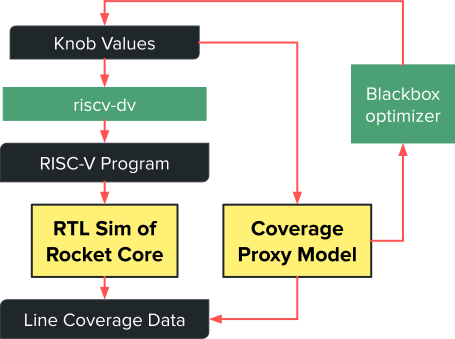
\includegraphics[width=0.65\linewidth]{figs/cov_proxy_model_usage.pdf}
  \caption{The verification loop enhanced with a coverage proxy model}
  \label{fig:cov_proxy_model}
\end{figure}

We used was a rocket-chip RV32IMC core as the RTL design.
We modified the testharness for this core with line coverage collection and dumping enabled and we used Verilator as the RTL simulator.

We defined a range of values that each knob can take on.
For integer knobs this was set based on intuition and for boolean knobs we permit 0 and 1.
Importantly, we also defined the default value for each knob and we only switch a knob assignment from its default with a certain probability.
This is done to avoid messing with too many knobs at once per configuration which would produce an unrealistic and splattered dataset.

Using this strategy, we sample 100 different knob configurations with a non-default probability per knob of 0.8.
For each knob configuration, we consider five different generator seeds, giving a total of 500 tests.
All the tests were run on the spike RISC-V ISA simulator for golden commit logs and also on the Verilator simulator.

\section{Results}

\subsection{Coverage Correlations}

We first look at the entire dataset on its own and figure out what the true dimensionality of each coverage vector is.
We collect hit counts for 8k unique coverpoints per test, but of those, 2.7k are never hit in the entire dataset, and 5k are hit by every test.
This leaves 470 coverpoints that actually have variance across different tests.

We first normalize each coverage count by the number of clock cycles it took to execute the test: the units are now (hits per cycle).
This is important because we don`t want to favor a test that has a larger cover count just because it runs for more simulation cycles.
In practice, to hit an RTL unit \textit{harder} to coax out bugs, we want to increase its hits/cycle, not aggregate hits alone.

Then, to construct the coverage correlation heatmap in figure \ref{fig:cov_heatmap}, we normalize each coverpoint`s hits/cycle by the maximum achieved by any test (so that each test`s strength for a given coverpoint is visible).

\begin{figure}
  %\centering
  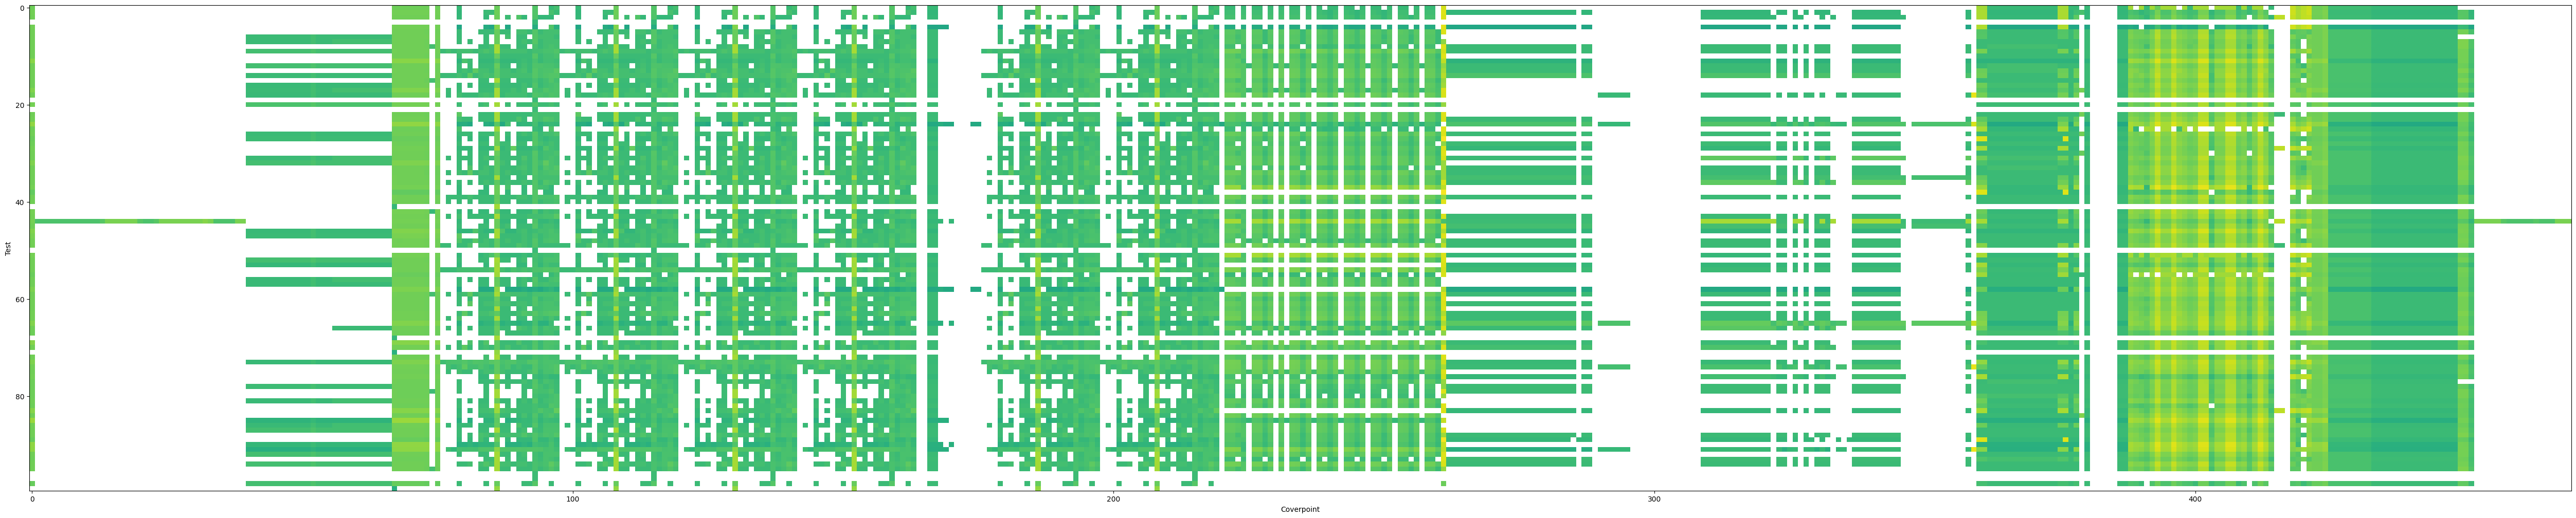
\includegraphics[width=\linewidth]{figs/cov_heatmap.png}
  \caption{A heatmap with each column representing one of 470 coverpoints and each row representing a single test (only 100 tests are shown). The more green a cell, the more aggressively that test hits the coverpoint with respect to all the other tests.}
  \label{fig:cov_heatmap}
\end{figure}

We can make these observations:

\begin{itemize}
  \item Many coverpoints are correlated with each other. This isn`t surprising for line coverage since a long if-elseif-else chain has predictable relationships based on which branches are taken. Also, if a test targets a particular unit, we expect many of the covers in that unit will be hit.
  \item Hitting certain coverpoints requires extreme luck or specific knob settings. For instance, the long thin row on the left represents coverpoints in the MMIO AXI4 interface. This interface will not be hit unless the core tries to access a specific memory region, which is completely up to chance (no knob control exists).
  \item If we take an SVD of this matrix, the first 1-3 singular values dominate, and the rest are close to 0. The real dimensionality of this matrix is not 470, but closer to 5 or 10.
\end{itemize}

\subsection{Proxy Model Evaluation}

We take a 80:20 train/test split several times and train a few different classical models (linear and ridge regressors and xgboost decision trees) to determine the typical model prediction accuracy.
While the mean absolute error does go down slightly from linear to ridge to xgboost models, the gain is marginal.

The mean / median absolute error is about \textbf{0.0004 / 5.24e-6 hits/cycle}.
In context, the median hits/cycle across all coverpoints is 5.43e-6 hits/cycle.
This is not a great result: the error margin is roughly equal to the value we`re trying to predict (median relative error across all coverpoints is close to 100\%).

See Figure \ref{fig:error_vs_seen_freq} for some analysis of the prediction error for a coverpoint as a function of how often that coverpoint was seen in the training set.
We would expect to see a negative correlation where increased incidence of a coverpoint would allow us to learn more about what knobs contribute to it.
However, we instead see no or even a slightly positive correlation.
This likely indicates that there is not enough training data or the data is too noisy for the model to learn anything.

\begin{figure}
  %\centering
  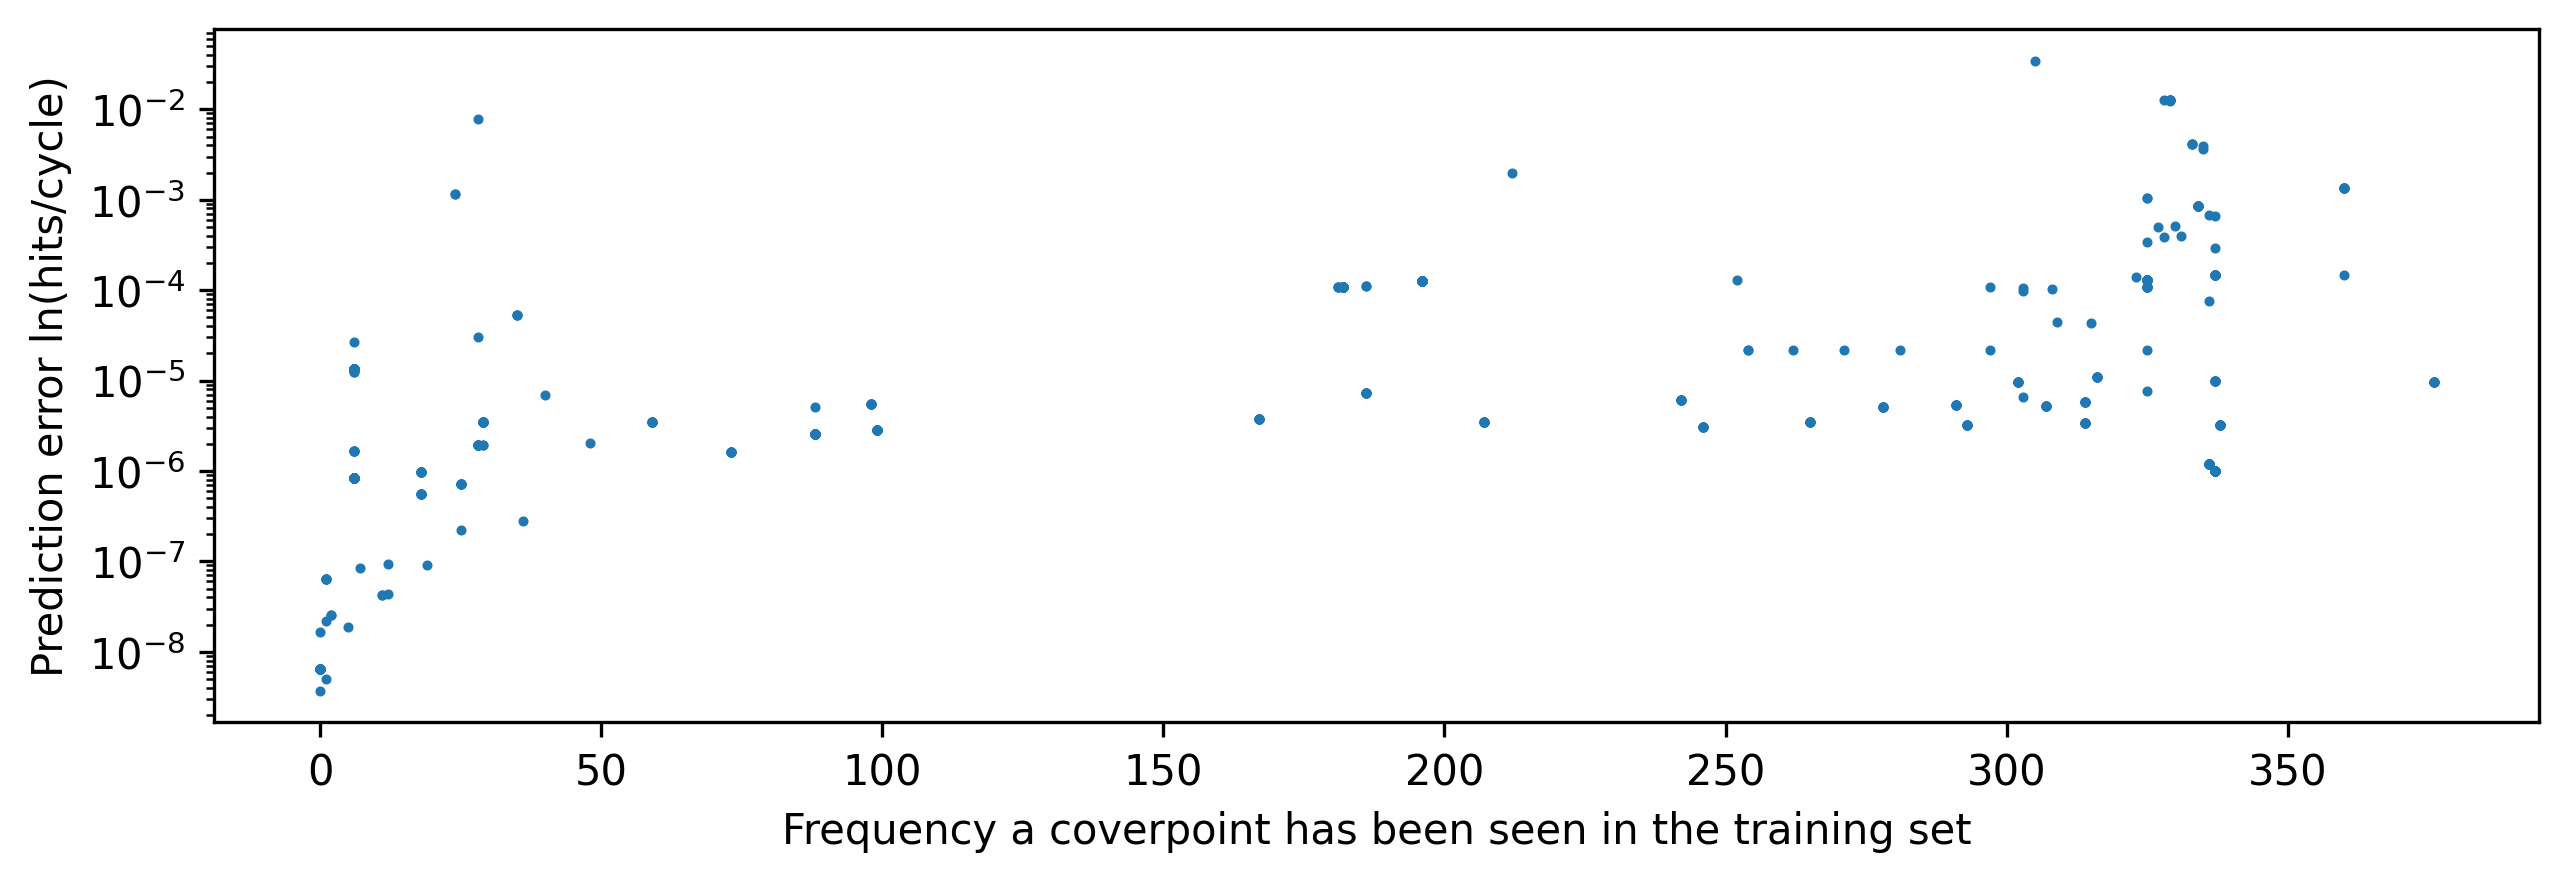
\includegraphics[width=\linewidth]{figs/error_vs_seen_freq.png}
  \caption{Coverpoint prediction error as a function of how frequently that coverpoint has been seen in the training set.}
  \label{fig:error_vs_seen_freq}
\end{figure}

\subsection{Variance of Coverpoint Hits By Seed}

We mentioned earlier that even with the same knob configuration, the seed passed into the simulator can also have an impact on the generated stimulus (and resultant coverage).
We attempt to visualize this in Figure \ref{fig:variance}.
It is clear that for some knob configurations, the seed has a large (25\%+) impact on hits and it is impossible for a model to predict that variance in a general way.

\begin{figure}
  %\centering
  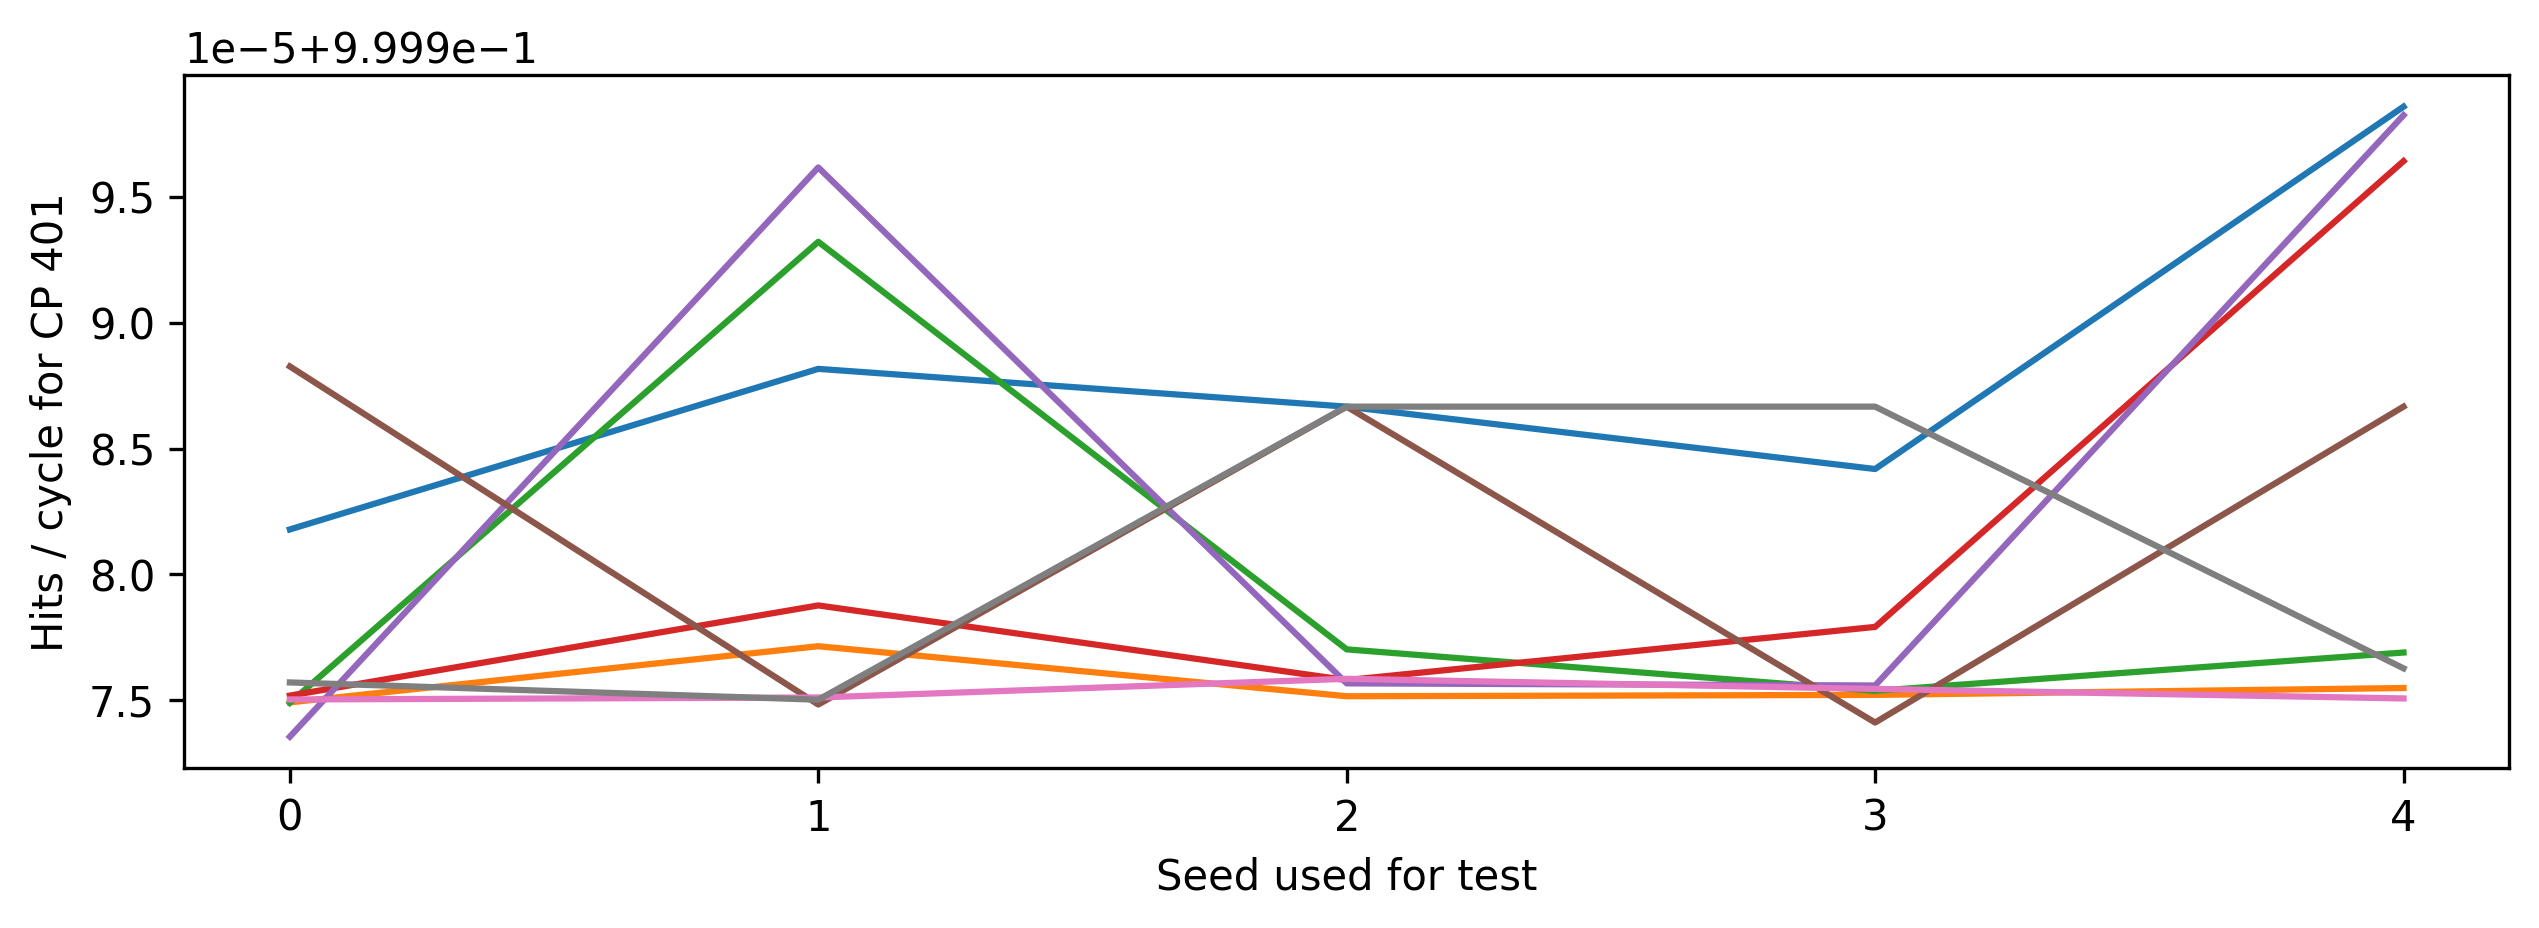
\includegraphics[width=\linewidth]{figs/variance2.png}
  \caption{Each different colored line represents a fixed knob configuration. The x-axis is the seed used for a run of the generator and the y-axis shows the hits/cycle for coverpoint 401 (picked arbitrarily).}
  \label{fig:variance}
\end{figure}

It is clear that riscv-dv makes many decisions that are not directly influenced by the knob values.
This limits the potential accuracy of any model using knob values alone as the input feature.

This motivates using more stimulus specific features such as the functional coverpoints included in riscv-dv.
We have a way to dump this generator-level coverage data, but work is still ongoing to parse that coverage database so its features can be used to embed a stimulus.

\subsection{Interpreting Model Weights}

One nice feature of classical AI models is their interpretability.
We take the ridge regression model and ask what is the most and least correlated knob with the following two coverpoints.

\begin{itemize}
  \item CP 10 (AXI4 to MMIO) - correlated with \verb|enable_misaligned_instr| and inversely with \verb|illegal_instr_ratio|
  \item CP 401 (ALU divider) - correlated with \verb|no_branch_jump| and inversely with \verb|set_mstatus_mprv|
\end{itemize}

These actually make some sense and can help validate that the model is at least learning something.

CP 10 is only hit when the core makes a memory request that accesses the MMIO physical address space.
It`s correlation with \verb|enable_misaligned_instr| is mysterious, but it`s inverse correlation with \verb|illegal_instr_ratio| is sensible since having more illegal instructions will cause the processor to spend time in trap handling code and with pipeline flushes rather than executing memory transactions.

CP 401 is hit whenever a RISC-V divide instruction is executed.
It makes sense that it is correlated with \verb|no_branch_jump| since disabling those control instructions increases the number of instructions riscv-dv can use for arithmetic ops, one of which is divide.
It`s inverse correlation with \verb|set_mstatus_mprv| also makes sense since trap handling code when dealing with memory privilege exceptions will consume the instruction budget over arithmetic ops.

\section{Discussion}

Overall, I think this work would have benefitted from constructing a larger dataset and from including generator-level functional coverage as an input feature.
Nevertheless, I have come to realize that perhaps riscv-dv is not architected in a way that is conducive for building coverage proxy models.

\subsection{Notes on riscv-dv}

Originally, I had planned on adding post randomization hooks to every class in riscv-dv so that I could capture the `decisions' the generator was making and use them as stimulus embedding features.
I realized that this is not viable since many riscv-dv classes perform additional mutation of class fields after randomization, and it is not possible to track the chain of function calls and mutable state.
This motivates an instruction generator that has fully controllable and natively instrumentable execution flow where we know what each byte of parametric randomness is used for.

Another note is that the tests produced by riscv-dv, across different knob configurations, do not have many distinguishing characteristics.
Coverage across different configurations is very similar, and many deviances are due to random seed selection and not knob value tuning.

Finally, we will note that the tens of knobs in riscv-dv provide very little control over the stimulus.
As the model weight analysis shows, most of the knob control that allows us to hit some coverpoints harder is actually just coincidental rather than a knob directly influencing a coverage outcome.

\subsection{Notes on Prior Work}

The most relevant prior work\cite{design2vec} attempts to train a coverage proxy model to classify coverpoints as hit or not hit.
This is a biased approach as simply increasing the number of instructions or different sequences in a test can increase the likelihood a coverpoint will be hit, even if it has nothing to do with specific knob settings.
We can observe in their supplemental materials that their model suggests the usage of \verb|instr_cnt| values about 10000 to hit certain coverpoints, when the default for that knob is 200.
It is very unlikely that hitting any coverpoint in a 3 stage Ibex core requires 10k instructions, so this seems to be an artifact of their predicted feature (hit/not hit vs hits/cycle) and the lack of control via knobs of riscv-dv.

\section{Future Work}

\subsection{Parametric Hardware Fuzzing}

This project has made clear that riscv-dv is not a suitable generator for training coverage proxy models or for attempting parametric fuzzing of hardware.
To that end, we are working on a QuickCheck-like library in Scala for describing stimulus generators that can handle hardware datatypes as well as declarative constraints specified as a Chisel circuit.

The idea is similar to QuickCheck in that at the core is a \texttt{Gen[T]} monad that describes how to generate a `random' value of type T, and we have a set of combinators for composing \texttt{Gen}s.
Once you have composed the entire generator monadically, you can invoke two different interpreters: one which delegates to the underlying Scala random stdlib, and an other which takes randomness from a stream of bytes which is user controllable.

Such a library would enable Zest-style fuzzing of hardware.
We are working on a RV32I instruction generator in this repo \url{https://github.com/girantinas/randomapi}.

\subsection{Coverage Extrapolation and RTL to Graph Conversion}

The prior work uses a coverpoint embedding in its coverage proxy model, but this requires learning the CP embedding along with the embedding of the knob values.
This means the CP embedding becomes design specific and requires retraining for new circuits.
However, it should be possible to start with a naive supervised coverage prediction model and then use a coverage extrapolation model to guess if any never before covered points might end up covered (Figure \ref{cov_extrapolation}).

The key infrastructure in testing this hypothesis is a RTL to graph compiler that can take as input RTL and emit a graph representation where all the connectivity, logic, and state information is preserved.
We are working on such a compiler for the FIRRTL hardware IR to emit a graph in the GML format in this repo \url{https://github.com/vighneshiyer/rtl2graph}.

\begin{figure}
  %\centering
  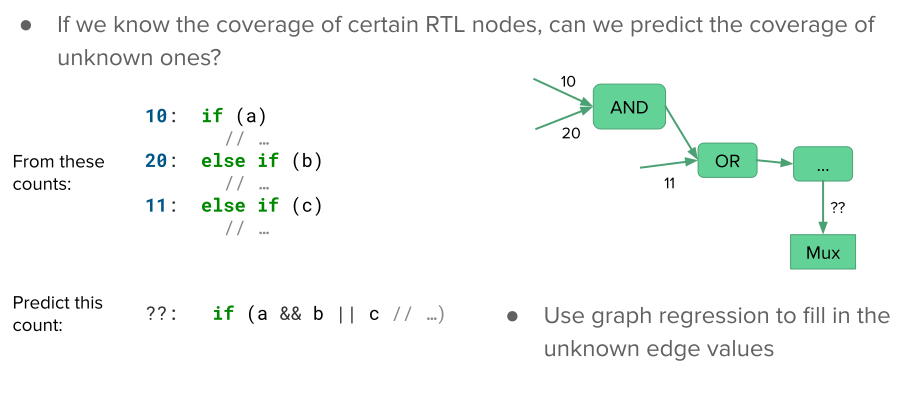
\includegraphics[width=\linewidth]{figs/cov_extrapolation.pdf}
  \caption{A potential approach to coverage extrapolation.}
  \label{fig:cov_extrapolation}
\end{figure}

\bibliographystyle{ACM-Reference-Format}
\bibliography{references}

\appendix

\end{document}
\endinput
